\documentclass{prova}

\usepackage{amssymb}
\usepackage[inline]{enumitem}

\newcommand{\sen}{\,\mbox{sen}\,}
\newcommand{\tg}{\,\mbox{tg}\,}
\newcommand{\cosec}{\,\mbox{cosec}\,}
\newcommand{\cotg}{\,\mbox{cotg}\,}
\newcommand{\tr}{\,\mbox{tr}\,}
\newcommand{\ds}{\displaystyle}
\newcommand{\ra}{\rightarrow}

\professor{Prof.\@ Adriano Barbosa}
\disciplina{C\'alculo Diferencial e Integral}
\avaliacao{PS}
\curso{Eng.\@ de Energia}
\data{26/07/2018}

\begin{document}
	\cabecalho{5}  % o numero 5 indica a qnt de quadros na tabela de nota

	\textbf{Todas as respostas devem ser justificadas.}

    \vspace{0.5cm}

    {\bf Avalia\c{c}\~ao P1:}
	\begin{questionario}
        \q{Calcule os limites:}
            \begin{questionario}
                \qq{$\ds\lim_{x\ra9} \frac{\sqrt{x}-3}{x-9}$}
                \qq{$\ds\lim_{x\ra3} \frac{\sqrt{x+6}-3}{x-3}$}
            \end{questionario}
        \q{Determine o maior dom\'{i}nio de $\ds f(x) = \frac{2x+1}{4x^2+4x+5}$ e os valores de $x$ para os quais $f$
            \'e cont\'{\i}nua.}
        \q{Calcule a derivada das fun\c{c}\~oes abaixo:}
            \begin{questionario}
                \qq{$\ds f(x) = \frac{1}{\sqrt{x}}-\frac{1}{\sqrt[3]{x}}$}
                \qq{$\ds f(x) = x^2\cos{(3x)}$}
            \end{questionario}
        \q{Dada $y=\cos{(\sen{(1+x^2)})}$. Calcule $\ds \frac{dy}{dx}$.}
        \q{Use deriva\c{c}\~ao impl\'{\i}cita para calcular $\ds \frac{dy}{dx}$, onde
            $2\sqrt{x}+\sqrt{y}=3$.}
	\end{questionario}

    \vspace{1cm}

    {\bf Avalia\c{c}\~ao P2:}
    \begin{questionario}
        \q{Ao meio dia o navio A est\'a 100km a oeste do navio B. Sabendo que o
            navio A viaja para sul a 35km/h e o navio B viaja para norte a
            25km/h, qu\~ao r\'apido eles est\~ao se distanciando as 16h?}
        \q{Encontre $f$ tal que $f''(t)=\sen{t}+\cos{t}$, $f(0)=3$ e
            $f'(0)=4$.}
        \q{Calcule a integral $\ds\int_0^4 (4-x)\sqrt{x}\ dx$.}
        \q{Qual a menor dist\^ancia vertical entre as par\'abolas $y=x^2+1$ e
            $y=x-x^2$?}

        \begin{figure}[h]
            \centering
            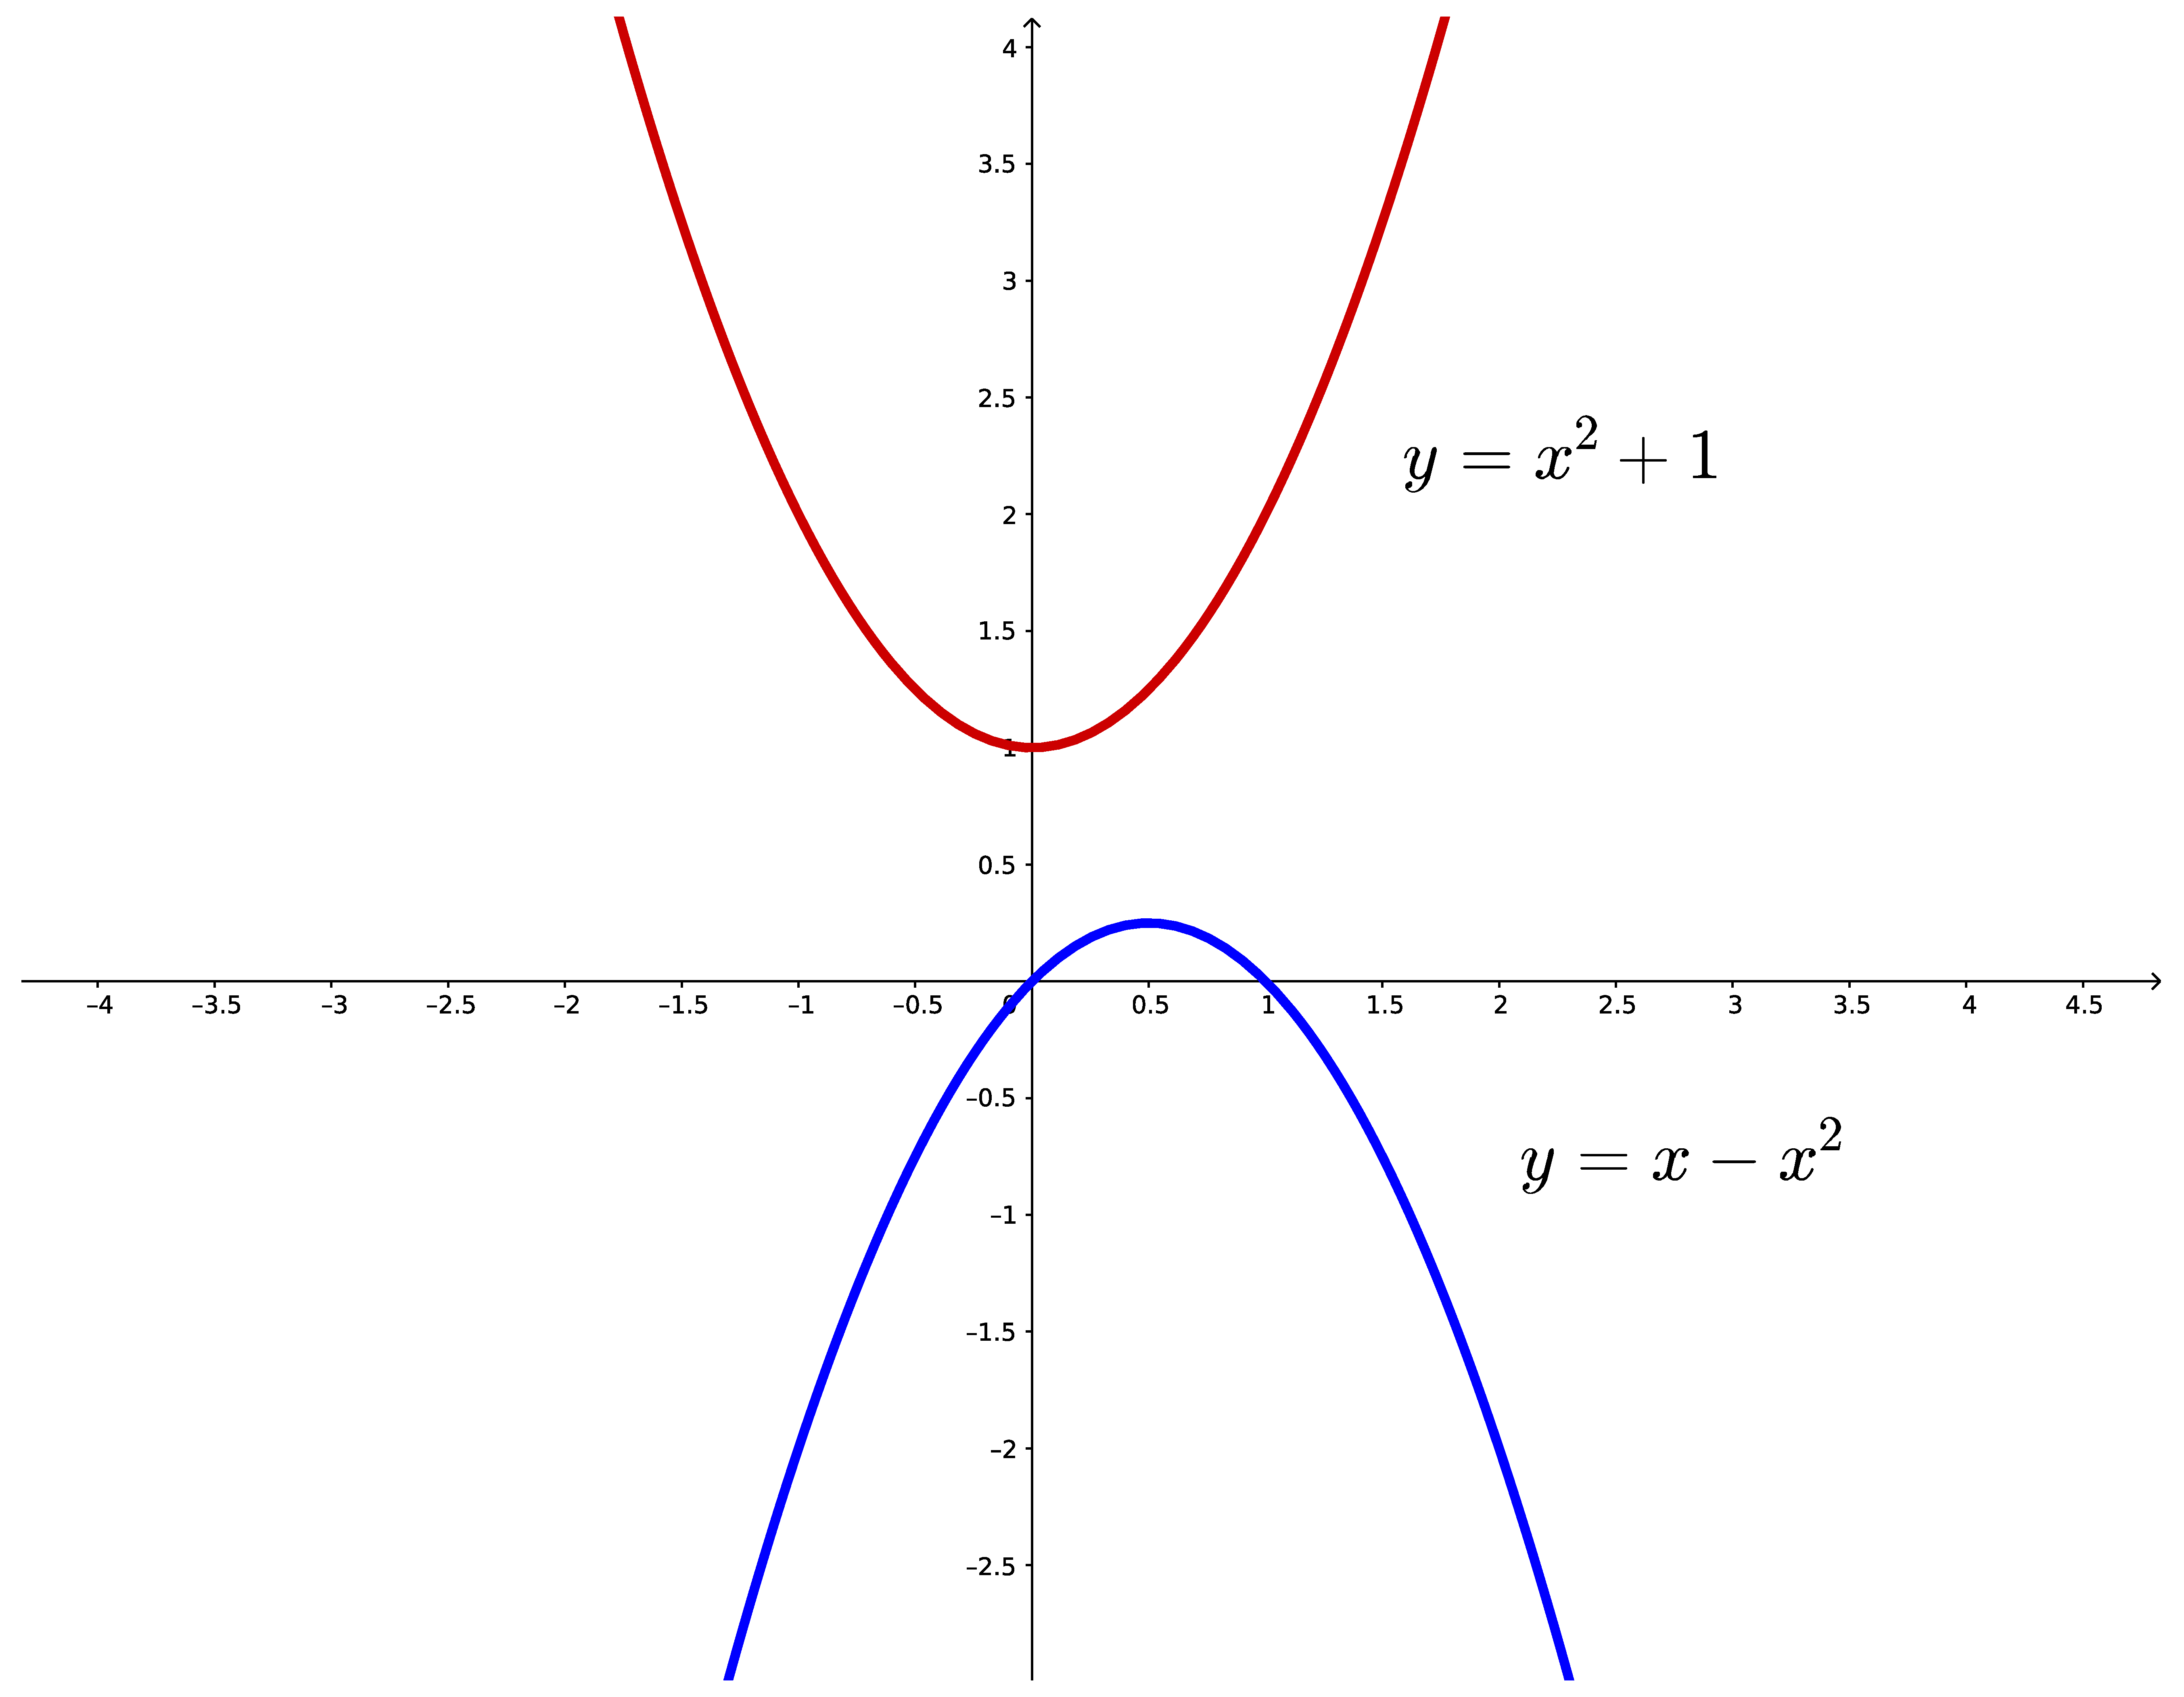
\includegraphics[width=0.6\textwidth]{grafico.pdf}
        \end{figure}

        \q{O gr\'afico de $f$ \'e dado abaixo. Calcule as integrais definidas:}
        \begin{figure}[h]
            \centering
            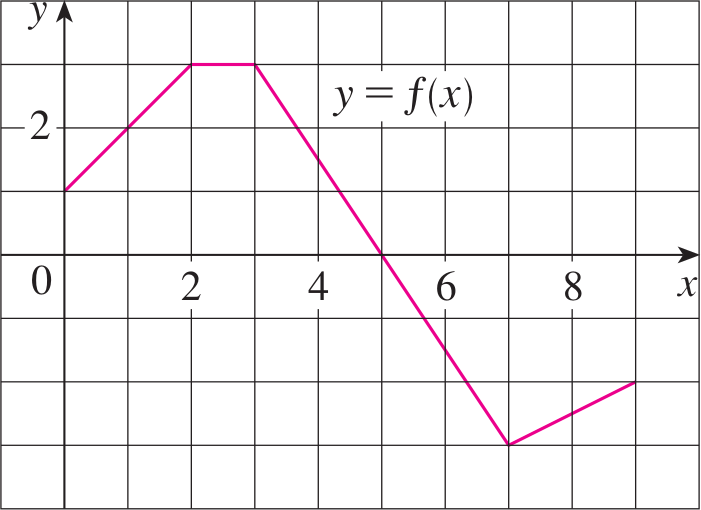
\includegraphics[width=0.4\textwidth]{area.png}
        \end{figure}

        \begin{enumerate*}
            \item $\ds \int_0^5 f(x)\ dx$
            \item $\ds \int_2^7 f(x)\ dx$
        \end{enumerate*}
    \end{questionario}
\end{document}
